\section{Introduction}
Carcassonne is a tile-based board game for two to five players.  The game board
is a medieval landscape built by the players as the game develops. There is a
initial tile on board, and abound 70 other tiles shuffled face down for the
players to draw from.  Each player takes turn to draw a tile and places it
adjacent to tiles that are already on board. The new tile must be placed in
such a way that extends the regions that is at the edge of the tiles it is
adjacent to.  In particular, roads must connect to roads, fields to fields and
cities to cities.  After placing a tile, the player can opt to place a
`follower' on a region of the newly-placed tile. The game ends when all the
tiles are placed.  At that time, each follower on board will be scored for
points according to the regions it is occupying. 
\begin{figure}[b]
\centering
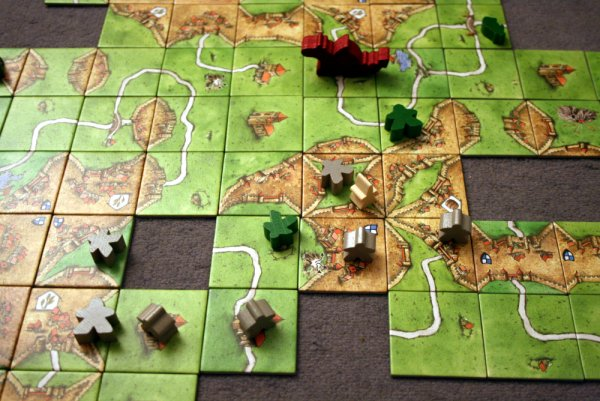
\includegraphics[height=.3\textheight]{board.jpg}
\caption{A part of a game board after several turns (image from
wikipedia).}
\label{fig:board}
\end{figure}
